% Methedology: 2,000 words

\chapter{Methodology}

The primary objective of our study is to develop an AI model using the technique of transfer-learning, to automatically predict RUST scores from an input radiograph. In this chapter, we will first discuss our model design, contextualising the choices that we made in choosing our classifier, optimizer, and pre-training datasets.\footnote{i.e. the datasets that are used to train the base model, before transfer-learning.} Next, we will discuss the primary datasets used in the study, before proceeding to the define the three protocols that we will conduct, and the hyperparameter tuning regime. Afterwards, the evaluation and endpoints will be presented, as well as a discussion on patient privacy and ethical considerations.

\section{Model Design}

Transfer learning is a technique which uses a model trained upon a larger dataset first, before being applied to a smaller, task-specific dataset. Assuming our task-specific dataset (in our case, the RUST data from METRC) is fixed, the performance of our transfer-learning model is determined by the following factors:

\begin{enumerate}
    \item The architecture of the original model.
    \item The initial, large dataset that the original model is trained on.
\end{enumerate}

\noindent
Hence, in the context of our study design, we must first choose (or create) a model architecture, and select an initial large dataset to train our model on. Only then are we able to apply the transfer learning procedure (e.g. freeze model weights, add new classifier, fine tuning, etc) upon our task-specific dataset.

\subsection{Model Architecture Choices}

The first decision that we must make in our experiment design is the choice of model architecture.
According to a literature survey by Litjens, Kooi, Bejnordi et al., convolutional neural networks (CNNs) are the most common deep learning architecture deployed for medical image analysis, vastly outnumbering alternative methods such as Stacked Autoencoders (SAE), or Recurrent Neural Networks (RNNs) \autocite[77]{cnn-most-common}.
This is expected, as CNNs exhibit strong performance with image classification tasks, and as our project is an image classification task (albeit with radiographs), we will be using a CNN.

The choice now remains to either design our own CNN from scratch, or use an existing CNN architecture.
Although designing a CNN \emph{ab initio} allows the possibility of further experimentation and potentially finer-grained control, such a \emph{de novo} model is difficult to assess holistically: there would be no prior work in literature to serve as a basis for comparison.
In contrast, if we use a well-documented, existing CNN as our transfer-learning foundation, we may compare the performance of our implementation against other instances of the same model architecture used for transfer-learning in different domains.
% The commensurability of a standard model for comparison is important: in a 2022 review of transfer learning techniques in medical image analysis, Kora, Ooi, Faust et al. found that only 13\% of prior studies compared their results with other models \autocite[94]{kora2022}. 

Thus, we will be using the InceptionV3 model, a convolutional neural network developed by Szegedy, Vanhoucke, Ioffe, et al.\ from Google \autocite{inceptionv3}. Our choice of InceptionV3 is based upon a 2022 literature review of transfer-learning models for the domain of medical image analysis. According to Kora, Ooi, Faust et al., CNNs with a broad (as opposed to deep) network topology perform well in transfer-learning tasks \autocite{kora2022}, with models like InceptionV3 outperforming more parameterized models like AlexNet \autocite{alexnet}. Indeed out of the 54 studies included in the review, Inception-style models both the most common (14 out of 54) and among the highest-performing. \autocite{kora2022}

\subsection{\enquote*{Top-Classifier} Choices}\label{sec:classifier}

Following the choice of our base model, we must then build a trainable classifier on top of the frozen base model layers. It will be the role of the classifier to transform the base model outputs into the 18-length one-hot encoded vector which will serve as our model's output. Top-classifiers are generally composed of a pooling layer, followed by layers of two or more densely interconnected neurons, with dropout. For our model, we have implemented the following classifier:

\begin{listing}[H]
    \begin{minted}[
        baselinestretch=1.0,
        frame=lines,
        mathescape,
        autogobble,
        fontsize=\footnotesize,
        style=default,
        breaklines,
        breakbytoken
    ]{python}
        classifier: tf.keras.Sequential = tf.keras.Sequential([
            layers.GlobalMaxPooling2D(),
            layers.Dense(1024, activation='relu'),
            layers.Dropout(dropout_rate),
            layers.Dense( 512, activation='relu'),
            layers.Dropout(dropout_rate),
            layers.Dense( 256, activation='relu'),
            layers.Dropout(dropout_rate),
            layers.Dense(  18, activation='sigmoid')
        ])
    \end{minted}
\caption{Classifier Architecture (\href{https://github.com/ShenZhouHong/radiography-ai-project/blob/cf8c9e9a1f07849787a98b2fc51df690354bf194/python/common/model.py}{Github})}\label{listing:classifier-def}
\end{listing}

\noindent
Our use of three \mintinline{python}{Dense} layers is fairly typical of classifiers built for transfer-learning applications. What does warrant a brief explanation, however --- is the choice of a \mintinline{python}{GlobalMaxPooling2D()} layer as a means to flatten the two-dimensional output of the base model. Why MaxPooling, instead of AveragePooling? We use MaxPooling because it \enquote*{selects} the brightest pixels per block-size. This performs well for images that are primarily composed of light pixels on dark backgrounds, such as our radiographs.

\subsection{Model Optimizer Choices}

Finally, the last architectural decision we must make in our model design, is the choice of an optimizer. We have two possible approaches: we may either select an optimizer from \emph{a priori} principles, or consider the selection of an optimizer to be a hyperparameter, and benchmark a variety of optimizers with our model on the data-set. Because we are already evaluating two variants of InceptionV3, the additional task of iterating through different optimizers will be infeasible given the time and compute constraints of the project.

Hence, our choice of an optimizer is determined by a review of available benchmarks and literature. The study and benchmarking of deep learning optimizers is a fairly recent field, initiated by the development of robust, reproducible benchmarks. Projects like Schneider, Balles, et Hennig's \emph{DeepOBS: A Deep Learning Optimizer Benchmark Suite} allowed researchers to evaluate optimizers against an assay of realistic optimization problems, simulating common deep learning tasks and neural network architectures. \autocite{deepobs} The availability of reproducible benchmarks allowed the first large-scale empirical experiments to be conducted on optimizer performance, culminating in Schmidt, Schneider, et Hennig's 2021 paper in optimizer benchmarking. \autocite{crowdedvalley} In an evaluation of 15 popular optimizers\footnote{AMSBound, AMSGrad, AdaBelief, AdaBound, AdaDelta, Adam, LookaheadMomentum, LookaheadRAdam, Momentum, NAG, NAdam, RAdam, RMSProp, and SGD, respectively. The full list of results are available in their supplementary appendix.} across a total of more than 50,000 epochs of training, significant data on optimizer performance was gathered.

Of the eight optimization problem assays in the benchmark suite, our task of radiographic image classification is bears closest resemblance to the CIFAR-10 benchmark: a CNN-based image classification task. According to the latest results available on the paper's website\footnote{\url{https://deepobs.github.io/leaderboardP4.html}}, the ADAM optimizer has a slight accuracy improvement over Momentum and SDG. However, the differences are so small that the author mentions: 

\blockcquote[2]{crowdedvalley}{
    \ldots\ a practitioner with a new deep learning task can expect to do about equally well by taking almost \emph{any method} from our benchmark and tuning it, as they would by investing the same computational resources into running a set of optimizers with their default settings and picking the winner.
}

\noindent
Therefore, we will select the ADAM optimizer, and spend time on fine-tuning the model and hyperparameter choices, instead of devoting further resources to selecting an optimizer.

\subsection{Pre-Training Dataset Choices}

Now that we decided our model architecture, the next step is to select the initial, or pre-training dataset, that is used to train the base model.

\subsubsection{ImageNet Dataset}
Originally, InceptionV3 was trained on the ImageNet dataset: a general-purpose collection of more than 14 million everyday images. \autocite{imagenet} The overwhelming size of the ImageNet dataset serves as a robust foundation for the InceptionV3 model, which exhibits strong performance in classification tasks upon it. However, the statistical characteristics of data in ImageNet is quite different from data in a typical radiography dataset. Hence, it remains a valid research question to ask whether a InceptionV3 model trained on a smaller, but more domain-specific dataset will exhibit better performance when applied to our transfer-learning task.

\subsubsection{RadImageNet Dataset}
Thus, we will also investigate RadImageNet, a collection of 5 million medical images composing of radiographic (CT), MRI, and ultrasound images. \autocite{radimagenet} As an open radiologic dataset developed specifically for transfer learning applications, a base model trained on RadImageNet may exhibit better performance on our radiography data, as the original network is trained upon images in a similar domain. However, the advantages of a similar domain is moderated by the corresponding smaller dataset size (5 million versus ImageNet's 14 million).

Therefore, in this project we will evaluate the use of a InceptionV3 model trained both on the ImageNet dataset, as well as the RadImageNet dataset as the base model for transfer learning. By comparing the performance of both models, we will be able to select the best-performing one for further development and refinement. 

% Additionally, the additional data point afforded by a second model allows greater context for our evaluation: according to Kora et al., only 13\% of transfer-learning studies benchmarked their model performance against a second model. \autocite[94]{kora2022} By choosing to evaluate two models from the very start of our project's design, we get to avoid this scientific blind-spot: and hopefully achieve a better result overall.

\section{Dataset}\label{sec:dataset}
% \section{Data Egress and Preprocessing}\label{sec:dataset}

Our transfer-learning models will be trained on a corpus of radiographic data sourced from a set of three METRC studies. \autocites{RetroDEFECT2022}{PAIN2017}{PACS2022} The data consists of pairs of radiographs (the anteroposterior view and the lateral view) along with a corresponding RUST score. 

% Now that we have defined the design of our experiment, we must define the pre-processing and data egress requirements.
% Our study data consists of anteroposterior and lateral view radiographs, as well as their corresponding RUST scores. This data is provided in a collaboration with METRC, Johns Hopkins University, through their archive of past and on-going studies. \autocites{RetroDEFECT2022}{OUTLET2021}{PAIN2017}{PACS2022} The data is held within REDCap: an electronic data and clinical trials database. \autocite{redcap} Because the data is held across multiple clinical trials and within multiple instruments, egressing data out of REDCap and pre-processing it into a useable form is a non-trivial software engineering task.

\begin{table}[H]
    \centering
    \begin{tabularx}{\textwidth}{@{}lXr@{}}
    \toprule
    \textbf{Dataset}     & \textbf{Name} & \textbf{Samples} \\ \midrule
    \autocite{RetroDEFECT2022} \textsc{RetroDEFECT} & \emph{Retrospective Study of the Treatment of Long Bone Defects}    & $1389$             \\
    \autocite{PAIN2017} \textsc{Pain}        & \emph{Pain Management \& Long Term Outcomes Following High Energy Orthopedic Trauma}      & $1233$             \\
    \autocite{PACS2022} \textsc{Pacs}        & \emph{Predicting Acute Compartment Syndrome using Optimized Clinical Assessment}    & $316$             \\ \midrule
    Sum         &      & $2938$            \\ \bottomrule
    \end{tabularx}%
    \caption{Sources of Radiographic Data with RUST labels in REDCap}\label{tab:datasets}
\end{table}

\noindent
The data is downloaded from the METRC Redcap database using the PyCap API library \autocite{pycap} and a set of Juypter notebooks (see Github repository link in \hyperref[sec:appendix-repo]{Appendix}), and then processed into a Tensorflow \mintinline{python}{tf.data.Dataset} object.

\subsection{One-Hot Encoding for Labels}

RUST Scores will be one-hot encoded as 18-length label Tensors. Recall that our model must predict a RUST score from a pair of input radiographs. RUST scores are measures of orthopaedic union (i.e. healing), and ordinarily consist of two subscores for each view (the anterior-posterior and medial-lateral views), quantifying the development of bone calluses and bridging over the fracture line. The score components are as follows:

\begin{table}[H]
    \centering
    \begin{tabular}{@{}ll@{}}
    \toprule
    Radiographic Feature              & Score \\ \midrule
    Fracture Line, No Callus          & 1     \\
    Fracture Line, Visible Callus     & 2     \\
    No Fracture Line, Bridging Callus & 3     \\
    No Fracture Line, Remodeled.      & 4     \\ \bottomrule
    \end{tabular}
    \caption{Radiographic Union Score for Tibial Fractures (RUST) Rubric}\label{tab:rust-score-components}
\end{table}

\noindent
These score components\footnote{Note that the original Whelan et al.\ paper \autocite{Whelan2010} does not include a value for remodelled fractures, however as the METRC dataset includes this category, we will be using the modified RUST variant specific to Johns Hopkins for this study.} are then used to assess the features of a fracture from the anterior, posterior, medial, and lateral cortices:

\begin{table}[H]
    \centering
    \begin{tabular}{@{}ll@{}}
    \toprule
                                   & Subscore \\ \midrule
    Anterior Cortex                &          \\
    Posterior Cortex               &          \\
    Medial Cortex                  &          \\
    Lateral Cortex                 &          \\ \bottomrule
    \end{tabular}
    \caption{RUST Scoring Instrument}\label{tab:rust-cortices}
\end{table}

\noindent
Finally the resulting subscore components are summed in order to yield a RUST score for the fracture as a whole.
For this study, our model is designed to predict every component subscore. Hence, the label will consist of a 18-value \mintinline{python}{tf.Tensor} with the shape (18,), consisting of 16 one-hot encoded values for the RUST subscores (four for each cortice), as well as two additional one-hot values to represent the view (anterioposterior or medial-lateral).

We explicitly choose to one-hot encode every component subscore of the RUST instrument in order to avoid bifurcating our already small dataset. Recall that it takes a pair of radiographs (one anteroposterior, one lateral) in order to score a fracture. If we chose to label each radiograph simply according to their component cortex sum (e.g. Anterior cortex score + Posterior cortex score), then we would have to develop two separate models, one for the anterioposterior views, and another for the lateral views. This would cut the effective size of our dataset in half, as there are two radiographs for every fracture.

% \subsection{Validate Radiography Data with Branch-Parser}

% The first challenge that we face in the data egress process, is finding RUST-radiography pairings that are valid for inclusion in our dataset. A small subset of radiographs do not possess valid RUST scores: either because they were uninterpretable due to hardware occlusion (e.g. presence of a titanium orthopaedic fixture), or because the radiograph was not taken for the purpose of assessing fracture healing. In order to validate the radiography data, a Python package called redcap-branch-parser was developed to parse the conditional logic contained within REDCap patient records. \autocite{redcap-branch-parser} The development of this package took up a non-trivial amount of early project work.

% Once valid RUST-radiograph pairs were identified, the study data was egressed out of REDCap using a set of ad-hoc Jupyter Notebooks and the PyCap API package. \autocite{pycap}

% \subsection{Automated de-skewing with ImageMagick}
% Following the egress of radiography data, the radiography image files were automatically de-skewed using ImageMagic. At this point, data-preprocessing is complete, as data augmentation will be performed dynamically via layers within Keras.

\subsection{Data Augmentation Strategy}

Because we have a small dataset, a robust data augmentation strategy is needed to combat overfitting. In order to develop our data augmentation strategy, we followed suggestions from Bejani et Ghatee's \emph{systematic review on overfitting control in shallow and deep neural networks} \autocite{overfitting-prevention}. We may categorise data augmentation strategies to three broad families of methods: \autocite{augmentation-strategies}

\begin{enumerate}
    \item \textbf{Geometric Methods:} rotation, cropping, flipping.
    \item \textbf{Photometric Methods:} noise, color-shifting, edge modification.
    \item \textbf{\enquote*{Complex} Methods:} generating artificial data using GANs, style transfer.
\end{enumerate}

\noindent
Of the three, \enquote*{complex} data augmentation methods such as generating artificial data points is inappropriate for our use case, as it will compromise the evidence-based labelling of our dataset. Hence, we may recourse to either geometric methods, or photometric methods. Originally, our intuition was that photometric data augmentation methods would be of limited applicability to radiographs, which are entirely greyscale. Upon further investigation, it turns out that when evaluated individually, the most effective data augmentation strategy is cropping and rotation. \autocite{benchmark} Our intuition was that cropping may not be appropriate, given that fracture-lines may lie on the peripheries of radiographs. Hence, we restrained ourselves to using only rotation, via random-flipping, as our method of data augmentation.

\section{Evaluation}

We will evaluate the performance of our models using a combination of K-fold cross-validation (for the initial evaluation and hyperparameter search), and a hold-out test set (for the final evaluation of the completed model).

\subsection{Performance Metric: AUROC}
The performance metric that we will be targetting is AUROC, the Area-Under-Curve of the Receiver Operating Characteristic (ROC) graph. This is the area underneath the precision-recall plot of the model, and is a common metric used to assess diagnostic accuracy. An AUROC of \(0.50\) indicates a diagnostic performance of no better than chance, while an AUROC of \(1.00\) indicates perfect performance.

\subsection{K-Fold Cross-Validation}
We will be using K-Fold Cross validation as a technique to get a more accurate assessment of our model performance. K-fold cross validation will be used during the initial evaluation of the different models (see \autoref{sec:protocols}), as well during hyperparameter search. We will be using a k value of \(k=10\) during the initial evaluation, and then a smaller k value of \(k=6\) for each sample of the hyperparameter space during the hyperparameter search (see \autoref{sec:hypersearch})

\begin{table}[H]
    \centering
    \begin{tabularx}{\textwidth}{@{}lll@{}}
    \toprule
    K-Fold & Percentage (of 3000) & Samples \\ \midrule
    6      & \(14\%\)             & 420     \\
    10     & \(8.5\%\)            & 255     \\ \bottomrule
    \end{tabularx}
    \caption{Size of validation set, per k-fold value.}\label{tab:k-fold-table}
\end{table}

% \noindent
% The value of \(k=10\) is chosen because the resulting per-fold training and validation splits are no larger than a conventional train, test, and validation split of 70\%, 15\%, 15\%, where:

% \begin{itemize}
%     \item Training and Validation Set (\texttt{ds\_train + ds\_valid}): 2490 (85\%):
%     \begin{itemize}
%         \item K-Fold Cross-Validation, $K$ = 10:
%         \begin{itemize}
%             \item Training Set:  2241  (\textasciitilde76\%)
%             \item Validation Set: 249  (\textasciitilde8.5\% per fold)
%         \end{itemize}
%     \end{itemize}
%     \item Hold-out Test Set (\texttt{ds\_test}): 441 (15\%)
% \end{itemize}

\noindent
Larger \(k\) values yield a more thorough measurement of a model's performance at the cost of additional computational costs, while lower \(k\) values risk lowering the training-validation split ratio until the training set is too small for adequate training. 

\subsection{Hold-Out Test Set}\label{sec:holdout-test-set}
A separate hold-out test set containing entirely unseen data will be reserved for a evaluation of the final model performance, after hyperparameter search. This hold-out test set will be kept strictly separate for final evaluation only, and will be used only once at the very end. With a dataset of \(\approx3,000\) samples, we will be setting aside \(15\%\) of the initial data (\(\approx450\) samples) for the hold-out test dataset.

\clearpage

\section{Protocols}\label{sec:protocols}

Now that we have finished discussing the model design, data, augmentation, and evaluation; it is time to define the study protocols. The experimental portion of this study will consist of three protocols:

\begin{enumerate}
    \item \hyperref[sec:protocol-i-method]{Protocol I}: Baseline: InceptionV3 end-to-end trained on RUST Dataset.
    \item \hyperref[sec:protocol-ii-method]{Protocol II}: Transfer-learning w/ InceptionV3 trained on ImageNet.
    \item \hyperref[sec:protocol-iii-method]{Protocol III}: Transfer-learning w/ InceptionV3 trained on RadImageNet.
\end{enumerate}

\noindent
All protocols will utilise the same data augmentation pipeline.

\begin{figure}[H]
    \centering
    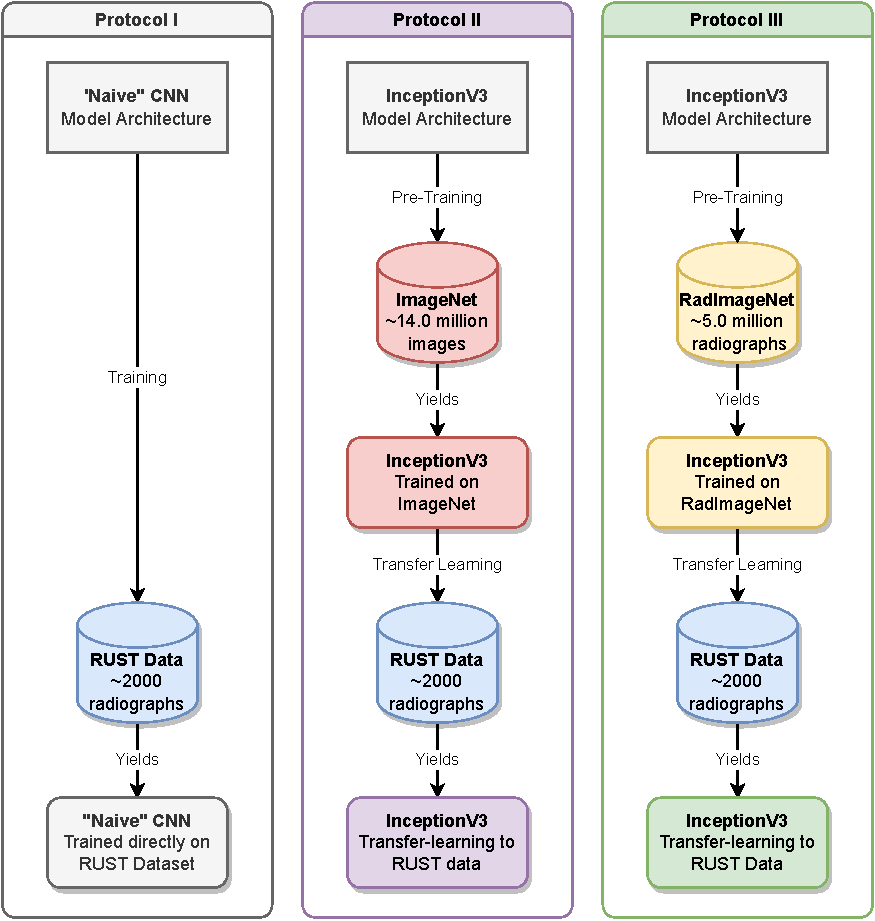
\includegraphics[
        page=1,
        width=\textwidth,
        angle=0,
        right
    ]{media/protocol-diagram.pdf}
    \caption{Overview illustrating the three model development protocols.}
    \label{fig:protocols}
\end{figure}

\subsection{Protocol I: InceptionV3 End-to-End Trained}\label{sec:protocol-i-method}

Protocol I is designed to help us establish a baseline level of performance that we will use to evaluate the feasibility of using transfer learning. Hence we will be using the same model architecture (InceptionV3) and classifier (see \autoref{sec:classifier}), but instead of using transfer-learning, we will train our model directly on the RUST dataset. We may expect a model that has only marginal performance, as the full InceptionV3 model has 23.9M trainable parameters \autocite{inceptionv3}, which will almost certainly not converge on a dataset of only 3000 samples. The performance of the Protocol I model will be used as a baseline for our subsequent investigations in transfer learning.

\noindent
The model will be evaluated using k-Fold cross-validation, with $k=10$.

\subsection{Protocol II: InceptionV3 with ImageNet}\label{sec:protocol-ii-method}

After establishing a baseline, we will move on to evaluating the use of ImageNet, or RadImageNet as our pre-training dataset for the transfer-learning model. Protocol II uses a base model (InceptionV3) with ImageNet weights. Here we use transfer-learning to train our classifier on the RUST dataset, and evaluate the AUROC of the resulting model using k-fold cross validation with \(k=10\).

\subsection{Protocol III: InceptionV3 with RadImageNet}\label{sec:protocol-iii-method}

Finally, we instantiate a third model that uses the InceptionV3 architecture, except this time our pre-training dataset is RadImageNet. Here we use transfer-learning on the InceptionV3 model with RadImageNet weights, to train our classifier on the RUST dataset once more, and evaluate the AUROC of the resulting model using k-fold cross-validation with \(k=10\).

Once this is complete, we will choose the better-performing model out of Protocols II and III (Protocol I's performance will almost certainly be marginal at best), and select it for further hyperparameter optimisation. This will take place according to two steps defined in the following section.

\section{Hyperparameter Search}\label{sec:hypersearch}

Using whichever is the better performing model, we will now attempt to optimise it's performance further by searching for better hyperparameters. We have the following hyperparameters that are available for consideration: \emph{dropout rate}, \emph{batch size}, \emph{learning rate}, and \emph{epsilon}.\footnote{A momentum factor similar to learning-rate decay specific to the Adam optimiser.} What is the best method for us to systematically find the best hyperparameters? A brief survey of machine learning literature informs us that a variety of methods are possible, including sophisticated approaches such as Bayesian optimization, and genetic algorithms. \autocite{yang2020} However, due to time and resource limitations we will be implementing only random search and grid search. We will perform a random search on the hyperparameter space defined by dropout and batch size, and then a grid search over a grid of different learning rates and epsilons.

This choice of performing hyperparameter search across two regimes is a practical compromise to the amount of compute resource that this project has. Although every hyperparameter influences every other hyperparameter, in practice it is rarely possible to conduct a hyperparameter search which varies over every hyperparameter under consideration at the same time. Instead, by constraining ourselves to two hyperparameters per search regime, we get to avoid the \enquote*{curse of dimensionality}\footnote{The concept in which the size of a hypothesis space grows combinatorially (\(n!\)) with the number of free parameters, i.e. degrees of freedom, which are added.}. Regime I is concerned with hyperparameters that are specific to the model, while Regime II is concerned with hyperparameters which are specific to the optimizer. Likewise, due to resource limitations, we will be performing k-fold cross validation for every search sample with a \(k=6\), instead of \(k=10\).

\subsection{Hyperparameter Search Regime I}\label{sec:regime-i}

Regime I uses a stochastic search process where the hyperparameter hypothesis space is randomly sampled \(t\) times. We use random search for Regime I because random search performs better than grid search over large hypothesis spaces, where the process of randomly sampling the hypothesis space will yield better hyperparameters as \(t\) increases, in a manner similar to Monte Carlo methods in statistics. \autocite{randomsearch} We begin by defining the range of batch size from \(16\) to \(2048\), and the range of possible dropout rates from \(0.00\) to \(0.50\).

Given this domain of batch size versus dropout, we will randomly sample the hypothesis space 100 times, where each sample contains a batch size and dropout rate pairing. Using this sampled pair, we will conduct a k-fold cross-validation experiment with \(k=6\), where for every experiment the model will be trained for \(20\) epochs with said hyperparameters. The resulting average AUROC across the k-fold cross validation experiment will be used to assess the performance of said hyperparameters.

\subsection{Hyperparameter Search Regime II}\label{sec:regime-ii}

After concluding Regime I, we will use the best-performing dropout and batch size, and proceed on to Regime II. Here, we aim to find the best learning rate and epsilon \(\epsilon\) (an Adam-specific momentum factor). Possible values for epsilon and learning rate span not merely a short interval (like those in Regime I), but across several orders of magnitude. Indeed, possible choices for learning rate can range from \(10^{-4}\) to \(10^{-1}\), while possible choices for epsilon can range from \(10^{-7}\) to \(10^{-1}\). Due to the sheer size of the search space, I judged random search to be infeasible. Instead, we will perform a grid search with a fixed set of learning rate and epsilon values, spanning each order of magnitude. 

Specifically, we will investigate the following learning rates: \(10^{-4}, 10^{-3}, 10^{-2}, 10^{-1}\) against the following epsilon values: \(10^{-7}, 10^{-6}, 10^{-5}, \ldots, 10^{-1}\).

\section{Research Questions and Final Evaluation}\label{sec:final-evaluation-method}

Once we have completed the Hyperparameter Search Regime II, we will have obtained the optimal set of batch size, dropout, learning rate, and epsilon for our model. Now will be the occasion for us to evaluate this final model against our hold-out test set (see \autoref{sec:holdout-test-set}). To do this, we will first train a new instance of our model with said optimal hyperparameters, observing its validation AUROC. Next, we will evaluate the model against the hold-out test set, and note the test AUROC.

Once we have done so, we will be able to answer the following research questions:
% First, prior to assessing model performance, we want to determine:

\begin{enumerate}
    \item \emph{Does Transfer-Learning using the InceptionV3 model perform better than end-to-end training with the InceptionV3 model?}
    \item \emph{Does the Transfer-Learning Model with the RadImageNet weights perform better than the Transfer-Learning Model with the ImageNet Weights?}
    \item \emph{Is Transfer-Learning able to achieve a persuasive level of performance, as measured by it's AUROC?}
\end{enumerate}

\noindent
Protocol I and Protocol II will allow us to answer questions one and two. Once we have found the best-performing variant of InceptionV3, we will then begin the process of optimising model performance as measured through AUROC. The final model, as evaluated on the hold-out test set, will be used to answer question three. For the purpose of this study, we define a persuasive level of performance as a final AUROC that is greater than or equal to \(0.80\).

% \begin{enumerate}
%     \item Endpoint 1: AUROC \(> 0.50\)
%     \item Endpoint 2: AUROC \(> \) End-to-End Model
%     \item Endpoint 3: AUROC \(\geq 0.80\)
% \end{enumerate}

% \noindent
% Initially, we aim to achieve an AUROC that is greater than chance, which is the minimal backstop to model performance. Failure to reach this endpoint will indicate severe flaws with our study design, such as our dataset being too small for even transfer-learning to be applicable. Following that, we want to exceed the performance of our \enquote*{naive} CNN. Finally, we wish to validate the concept of using AI to infer RUST scores from radiographs, by achieving an AUROC that is greater than 0.75.

% \section{Feasibility and Proof of Concept}

% Right now, a significant and on-going challenge is completing the initial data egress and pre-processing. As the study dataset is still not assembled and ready to use yet, initial feasibility and proof of concept experiments can be conducted on a readily available dataset from a similar domain, such as the MURA musculoskeletal radiography data from Stanford. By beginning with an artificially constrained subset of images and labels from MURA, we may validate our transfer learning protocol and gather some preliminary information.

% \subsection{Experiments with the MURA Dataset}
% \emph{This subsection is unavailable in this version of the document.}

% \subsection{Preliminary Results}
% \emph{This subsection is unavailable in this version of the document.}

\section{Ethical Considerations}

Any research project or study that involves human subjects will necessitate ethical consideration. This section is only a brief discussion of ethical risks and mitigations. The aim of this project is to validate transfer learning as a technique to infer RUST scores from a small dataset of radiographs. Although we aim to achieve robust performance in order to demonstrate the feasibility of this technique as an avenue for further research, at no time do we imply to develop a \emph{diagnostic} tool for clinical use. The overarching spirit of the study is to explore interdisciplinary applications of AI in medical imaging, in hopes of reducing clinical caseload for medical practitioners, leading to better standards of care for all patients overall. This study has passed Goldsmiths IRB review.

\subsection{Human Subject Research, and HIPAA Compliance}
This study works with radiographs collected from human subjects, that were a part of past or on-going METRC studies in high-energy trauma. This data is fully anonymised, and does not contain any personally identifiable information. As a part of Johns Hopkins Bloomberg School of Public Health's IRB requirements, all researchers working with human data, even anonymised data, must complete a Human Subject Research certification, and a Information Privacy Security certification. The author of this paper attests that they hold the aforementioned qualifications (see Appendix, \hyperref[sec:compliance]{Human Research Certification}).